\fancyhead[L]{\textbf{\textsf{64}}\quad \textbf{\textsf{CHƯƠNG 1}}\quad \textsf{Hàm số và Mô hình}}
\fancyhead[R]{}

\noindent
\begin{minipage}[t]{0.26\textwidth}
    \vspace{0pt}
    \centering
    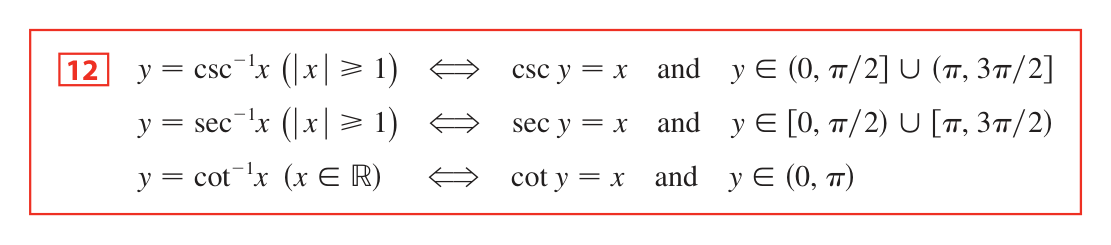
\includegraphics[width=\linewidth]{images/p0099_fig1.png}\\[4pt]
    {\raggedright\small\textbf{\textsf{HÌNH 26}}\\$y = \sec x$\par}
\end{minipage}%
\hfill
\begin{minipage}[t]{0.71\textwidth}
    \vspace{0pt}
    Ta biết rằng các đường thẳng $x = \pm\pi/2$ là các tiệm cận đứng của đồ thị hàm số $\tan$. Vì đồ thị của $\tan^{-1}$ nhận được bằng cách lấy đối xứng đồ thị của hàm tang thu hẹp qua đường thẳng $y = x$, nên suy ra các đường thẳng $y = \pi/2$ và $y = -\pi/2$ là các tiệm cận ngang của đồ thị $\tan^{-1}$.

    Các hàm số lượng giác ngược còn lại ít khi được sử dụng hơn và được tóm tắt ở đây.

    \vspace{0.41em}
    \begin{tcolorbox}[colframe=stewartred, colback=white, boxrule=1.2pt, arc=0mm, left=6pt, right=6pt, top=6pt, bottom=6pt]
        \begin{tabular}{@{}c@{\quad}l@{}}
            \tcbox[colback=white, colframe=stewartred, boxrule=1pt, sharp corners, size=small]{\color{stewartred}\textbf{12}} &
            $\begin{aligned}
                y &= \csc^{-1} x\ (|x| \ge 1) &\iff& \csc y = x \quad\text{và}\quad y \in (0, \pi/2] \cup (\pi, 3\pi/2] \\
                y &= \sec^{-1} x\ (|x| \ge 1) &\iff& \sec y = x \quad\text{và}\quad y \in [0, \pi/2) \cup [\pi, 3\pi/2) \\
                y &= \cot^{-1} x\ (x \in \mathbb{R}) &\iff& \cot y = x \quad\text{và}\quad y \in (0, \pi)
            \end{aligned}$
        \end{tabular}
    \end{tcolorbox}
    \vspace{0.25em}

    Việc lựa chọn các khoảng cho $y$ trong định nghĩa của $\csc^{-1}$ và $\sec^{-1}$ chưa có sự thống nhất chung giữa các tác giả. Chẳng hạn, một số tác giả dùng $y \in [0, \pi/2) \cup (\pi/2, \pi]$ trong định nghĩa của $\sec^{-1}$. [Bạn có thể quan sát đồ thị của hàm secant ở Hình 26 để thấy rằng cả sự lựa chọn này lẫn lựa chọn trong (12) đều hoàn toàn phù hợp.]
\end{minipage}

\vspace{1.23em}

% Dòng tiêu đề mục Bài tập
\noindent
{\color{stewartcyan}\rule{0.18\textwidth}{2pt}}\hspace{0.02\textwidth}%
{\LARGE\textbf{\textsf{\color{stewartcyan}1.5}}}\quad {\LARGE\textbf{\textsf{Bài tập}}}\hspace{0.02\textwidth}%
{\color{stewartcyan}\rule{0.53\textwidth}{2pt}}

\vspace{0.82em}

\noindent
\begin{minipage}[t]{0.48\textwidth}
    \begin{enumerate}[label=\textbf{\arabic*.}, leftmargin=*]
        \item \begin{enumerate}[label=(\alph*), leftmargin=*]
            \item Hàm số đơn ánh (hàm một--đối--một) là gì?
            \item Làm thế nào để biết một hàm số có phải là hàm đơn ánh hay không thông qua đồ thị của nó?
        \end{enumerate}

        \item \begin{enumerate}[label=(\alph*), leftmargin=*]
            \item Giả sử $f$ là một hàm đơn ánh có tập xác định $A$ và tập giá trị $B$. Hàm ngược $f^{-1}$ được định nghĩa như thế nào? Tập xác định của $f^{-1}$ là gì? Tập giá trị của $f^{-1}$ là gì?
            \item Nếu biết công thức của hàm số $f$, làm cách nào để tìm công thức của hàm ngược $f^{-1}$?
            \item Nếu biết đồ thị của hàm số $f$, làm cách nào để tìm đồ thị của hàm ngược $f^{-1}$?
        \end{enumerate}
    \end{enumerate}

    \noindent
    {\color{stewartcyan}\textbf{3--16}}\; Mỗi hàm số sau đây được cho bởi một bảng giá trị, đồ thị, công thức hoặc mô tả bằng lời. Hãy xác định xem hàm số đó có phải là đơn ánh hay không.

    \vspace{0.66em}
    \noindent
    \textbf{3.}\quad
    \begin{tabular}{|c|c|c|c|c|c|c|}
        \hline
        $x$ & 1 & 2 & 3 & 4 & 5 & 6 \\ \hline
        $f(x)$ & 1.5 & 2.0 & 3.6 & 5.3 & 2.8 & 2.0 \\ \hline
    \end{tabular}

    \vspace{0.66em}
    \noindent
    \textbf{4.}\quad
    \begin{tabular}{|c|c|c|c|c|c|c|}
        \hline
        $x$ & 1 & 2 & 3 & 4 & 5 & 6 \\ \hline
        $f(x)$ & 1.0 & 1.9 & 2.8 & 3.5 & 3.1 & 2.9 \\ \hline
    \end{tabular}

    \vspace{0.82em}
    \noindent
    \begin{minipage}[t]{0.48\linewidth}
        \textbf{5.}\\[4pt]
        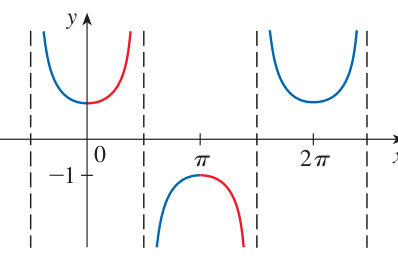
\includegraphics[width=\linewidth]{images/p0099_fig2.png}
    \end{minipage}\hfill
    \begin{minipage}[t]{0.48\linewidth}
        \textbf{6.}\\[4pt]
        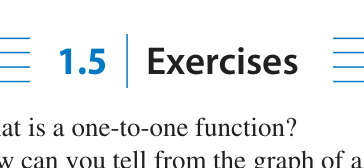
\includegraphics[width=\linewidth]{images/p0099_fig3.png}
    \end{minipage}

    \vspace{0.82em}
    \noindent
    \begin{minipage}[t]{0.48\linewidth}
        \textbf{7.}\\[4pt]
        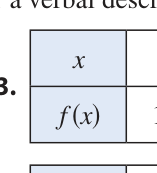
\includegraphics[width=\linewidth]{images/p0099_fig4.png}
    \end{minipage}\hfill
    \begin{minipage}[t]{0.48\linewidth}
        \textbf{8.}\\[4pt]
        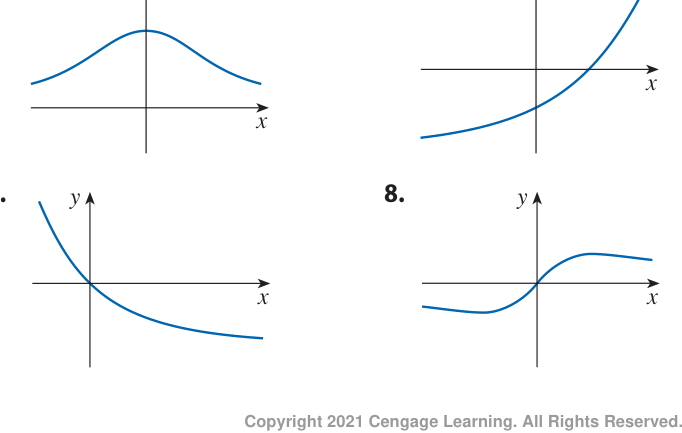
\includegraphics[width=\linewidth]{images/p0099_fig5.png}
    \end{minipage}
\end{minipage}%
\hfill
\begin{minipage}[t]{0.48\textwidth}
    \noindent
    \begin{minipage}[t]{0.48\linewidth}
        \textbf{9.} $f(x) = 2x - 3$\\[6pt]
        \textbf{11.} $r(t) = t^3 + 4$\\[6pt]
        \textbf{13.} $g(x) = 1 - \sin x$
    \end{minipage}\hfill
    \begin{minipage}[t]{0.48\linewidth}
        \textbf{10.} $f(x) = x^4 - 16$\\[6pt]
        \textbf{12.} $g(x) = \sqrt[3]{x}$\\[6pt]
        \textbf{14.} $f(x) = x^4 - 1, \quad 0 \le x \le 10$
    \end{minipage}

    \vspace{0.66em}
    \noindent
    \textbf{15.} $f(t)$ là độ cao của quả bóng đá sau cú phát bóng $t$ giây.

    \vspace{0.33em}
    \noindent
    \textbf{16.} $f(t)$ là chiều cao của bạn ở độ tuổi $t$.

    \vspace{0.41em}
    \noindent
    {\color{stewartcyan}\rule{\linewidth}{1pt}}
    \vspace{0.41em}

    \begin{enumerate}[label=\textbf{\arabic*.}, leftmargin=*, resume*]
        \setcounter{enumi}{16}
        \item Giả sử $f$ là một hàm đơn ánh.
        \begin{enumerate}[label=(\alph*), leftmargin=*]
            \item Nếu $f(6) = 17$, thì $f^{-1}(17)$ bằng bao nhiêu?
            \item Nếu $f^{-1}(3) = 2$, thì $f(2)$ bằng bao nhiêu?
        \end{enumerate}

        \item Nếu $f(x) = x^5 + x^3 + x$, hãy tìm $f^{-1}(3)$ và $f(f^{-1}(2))$.

        \item Nếu $g(x) = 3 + x + e^x$, hãy tìm $g^{-1}(4)$.

        \item Cho đồ thị của hàm số $f$ như hình vẽ bên dưới.
        \begin{enumerate}[label=(\alph*), leftmargin=*]
            \item Tại sao $f$ là hàm đơn ánh?
            \item Tìm tập xác định và tập giá trị của $f^{-1}$.
            \item Giá trị của $f^{-1}(2)$ bằng bao nhiêu?
            \item Hãy ước lượng giá trị của $f^{-1}(0)$.
        \end{enumerate}
    \end{enumerate}

    \begin{center}
        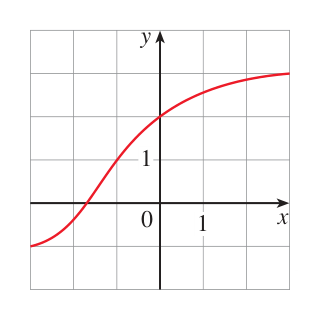
\includegraphics[width=0.45\linewidth]{images/p0099_fig6.png}
    \end{center}

    \noindent
    \textbf{21.} Công thức $C = \frac{5}{9}(F - 32)$, với $F \ge -459{,}67$, biểu thị nhiệt độ Celsius $C$ theo nhiệt độ Fahrenheit $F$. Hãy tìm công thức của hàm ngược và nêu ý nghĩa thực tế của nó. Tập xác định của hàm ngược là gì?
\end{minipage}